\setlength{\unitlength}{1pt}%
\makeatletter%
\let\ASYencoding\f@encoding%
\let\ASYfamily\f@family%
\let\ASYseries\f@series%
\let\ASYshape\f@shape%
\makeatother%
\leavevmode\vbox to 107.391970pt{}%
\kern 148.545630pt%
\special{pdf:0.000000 g}%
\special{pdf:0.000000 G}%
\fontsize{12.000000}{14.400000}\selectfont%
\usefont{\ASYencoding}{\ASYfamily}{\ASYseries}{\ASYshape}%
\ASYalign(-74.272815,53.695985)(-0.500000,-0.500000){\hbox to 0pt{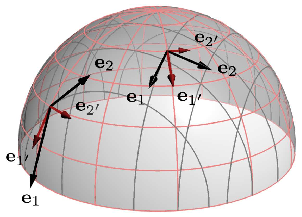
\includegraphics[hiresbb]{./figuras/hemisferio_norte_S2+0_0.pdf}\hss}%
\includemedia[noplaybutton,3Dlights=Headlamp,3Dmenu,3Dtoolbar=false,label=hemisferio_norte_S2,3Daac=16.185188108,3Dc2w=0.389418342 -0.921060994 0 -0.342073466 -0.144626342 0.928476691 -0.855183664 -0.361565854 -0.371390676 316.916786788 130.937408341 155.286569621,3Droo=362.280587463,3Dpsob=H,3Dbg=1 1 1,add3Djscript=asylabels.js]{\phantom{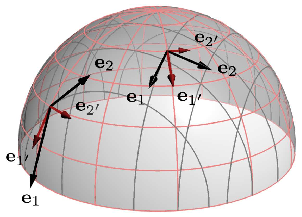
\includegraphics[hiresbb]{./figuras/hemisferio_norte_S2+0_0.pdf}}}{./figuras/hemisferio_norte_S2+0.prc}}%
